% !TEX root = main.tex
\documentclass[a4paper, UKenglish, 11pt]{uiomaster}
\usepackage{lipsum}
\usepackage[subpreambles=true]{standalone}
\usepackage[table,xcdraw]{xcolor}
\usepackage{placeins}

% discuss how this is not 3d, but 2d ??

\begin{document}
\chapter{Convolutional Neural Network Approach for Localizing Single Dipole Sources} \label{chap:simple_dipole_CNN}
\chaptermark{CNN for Localizing Single Dipole Sources}
In this chapter, we explore the utilization of a Convolutional Neural Network (CNN) for the task of localizing simple current dipoles from EEG recordings. The CNN is a type of feed-forward neural network that excels at learning spatial features from images. The objective of this investigation is to assess whether leveraging spatial information in EEG recordings as images can enhance a neural network's ability to analyze EEG data and yield more accurate predictions for localizing the sources generating the neural signals.

\rednote{Fix citing.}
\section{Adjusting the Data Set}
Convolutional Neural Networks are well-known for their effectiveness in processing image data. Images share an intrinsic structure. Commonly they are stored as three-dimensional arrays; with an width axis, height axis and what is commonly referred to as a \emph{channel axis}. In image data, the number of channels a pixel has determines how many values are needed to describe its color. A standard RGB image holds three distinct channels used to specify the color of the pixel, while for a grayscale image, there is only one channel used to specify the brightness of that pixel.

In order to utilize CNNs for EEG data analysis, we perform an \emph{interpolation} process on the original data set presented in Chapter 3. Interpolation is a mathematical technique that estimates values between known data points, effectively filling in the gaps by providing approximations for unobserved data points. By applying interpolation to our EEG data, we create a representation resembling the structure of an image. This transformation converts the original one-dimensional EEG data into a regular 2D grid format, imparting image-like characteristics while preserving spatial structures.

% means that when you have data points at certain positions, interpolation can fill in the gaps by providing estimated values for positions or data points that were not originally observed or measured.
The resulting data is represented as a 20x20x1 array, mirroring the structure of a grayscale image. Within this array, each element stores the intensity value of the EEG potential recorded at a specific spatial location. Unlike traditional grayscale images where pixel values convey color intensity, in our context, each pixel's value signifies the intensity of the recorded EEG signal at the corresponding position. This representation may empower the CNN to leverage the spatial arrangement of the EEG data, uncover relevant patterns, and discern local relationships, similar to the way CNNs process conventional image data.

By preserving these spatial structures, we hope for the network to effectively utilize local relationships among neighboring recording electrodes. For instance, when one electrode records a high EEG value, the inherent data patterns suggest that nearby electrodes should also register relatively high EEG values due to their close spatial proximity. These spatial relationships may expedite the network's training compared to the simpler fully connected feed-forward neural network (FCNN), as it efficiently captures meaningful representations by harnessing these inherent patterns.

Figure \ref{fig:eeg_dipole_pos_0} illustrates the process of interpolation. The right panel shows scatter plots of samples from the original data, where the EEG data is plotted at corresponding electrode locations at the scalp seen from above ($xy$-plane). Each measuring electrode is depicted as a circle holding the EEG recording at that specific electrode. The middle and left panels display the contour plots of the original EEG data and the interpolated data, respectively. The contour plot of the interpolated data illustrates how the input data for the convolutional neural network is organized in an image-like manner.

\begin{figure}[!htb]
\centering
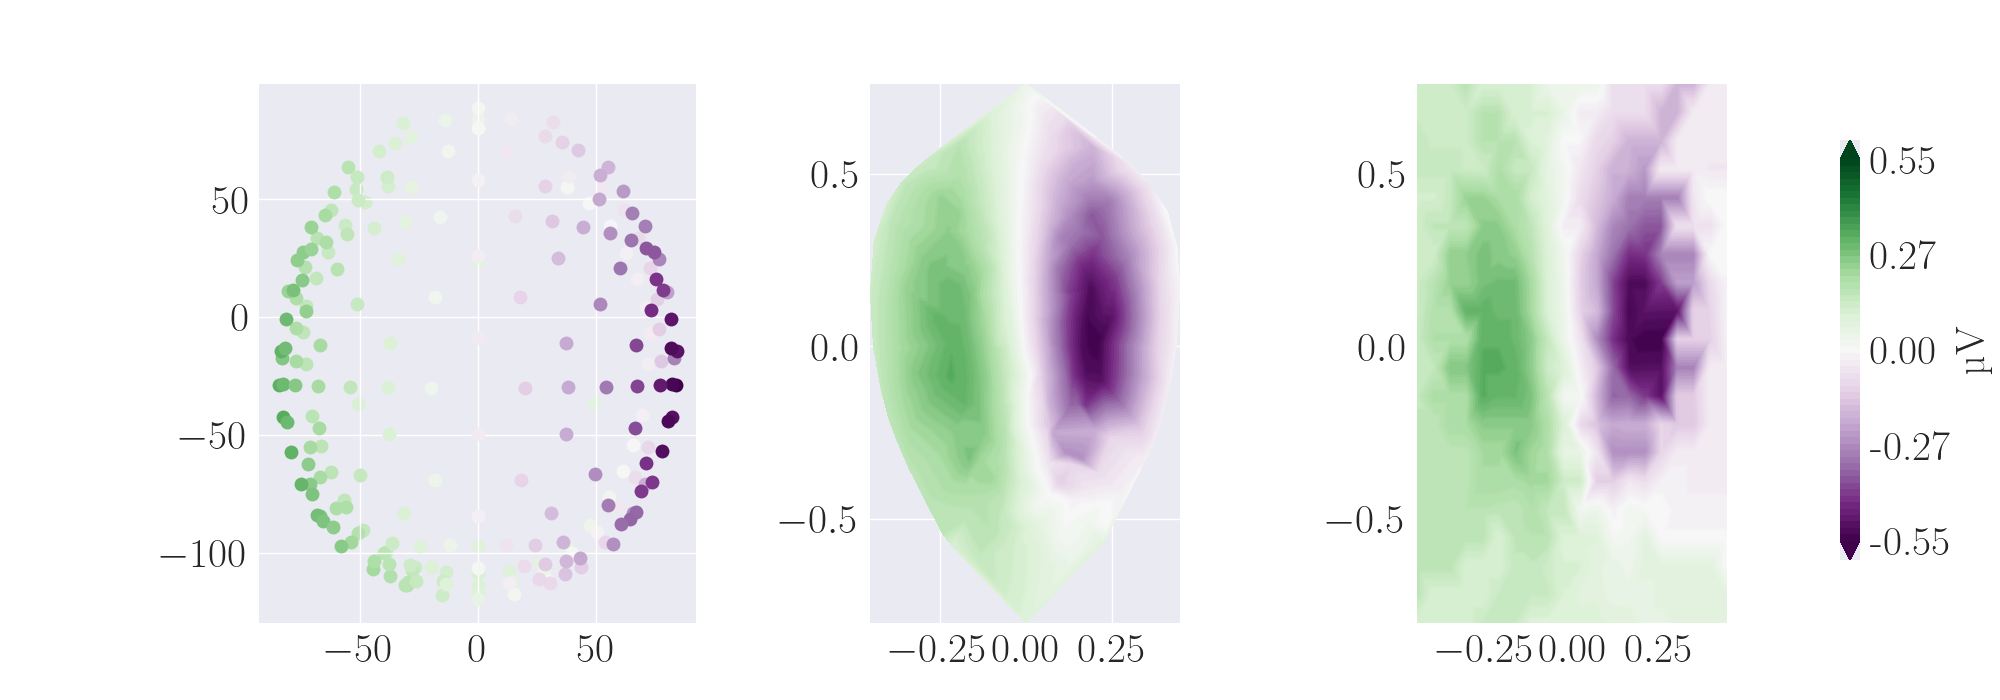
\includegraphics[width=\linewidth]{figures/purple_green/one_dipole_eeg_dipole_pos_0.png}
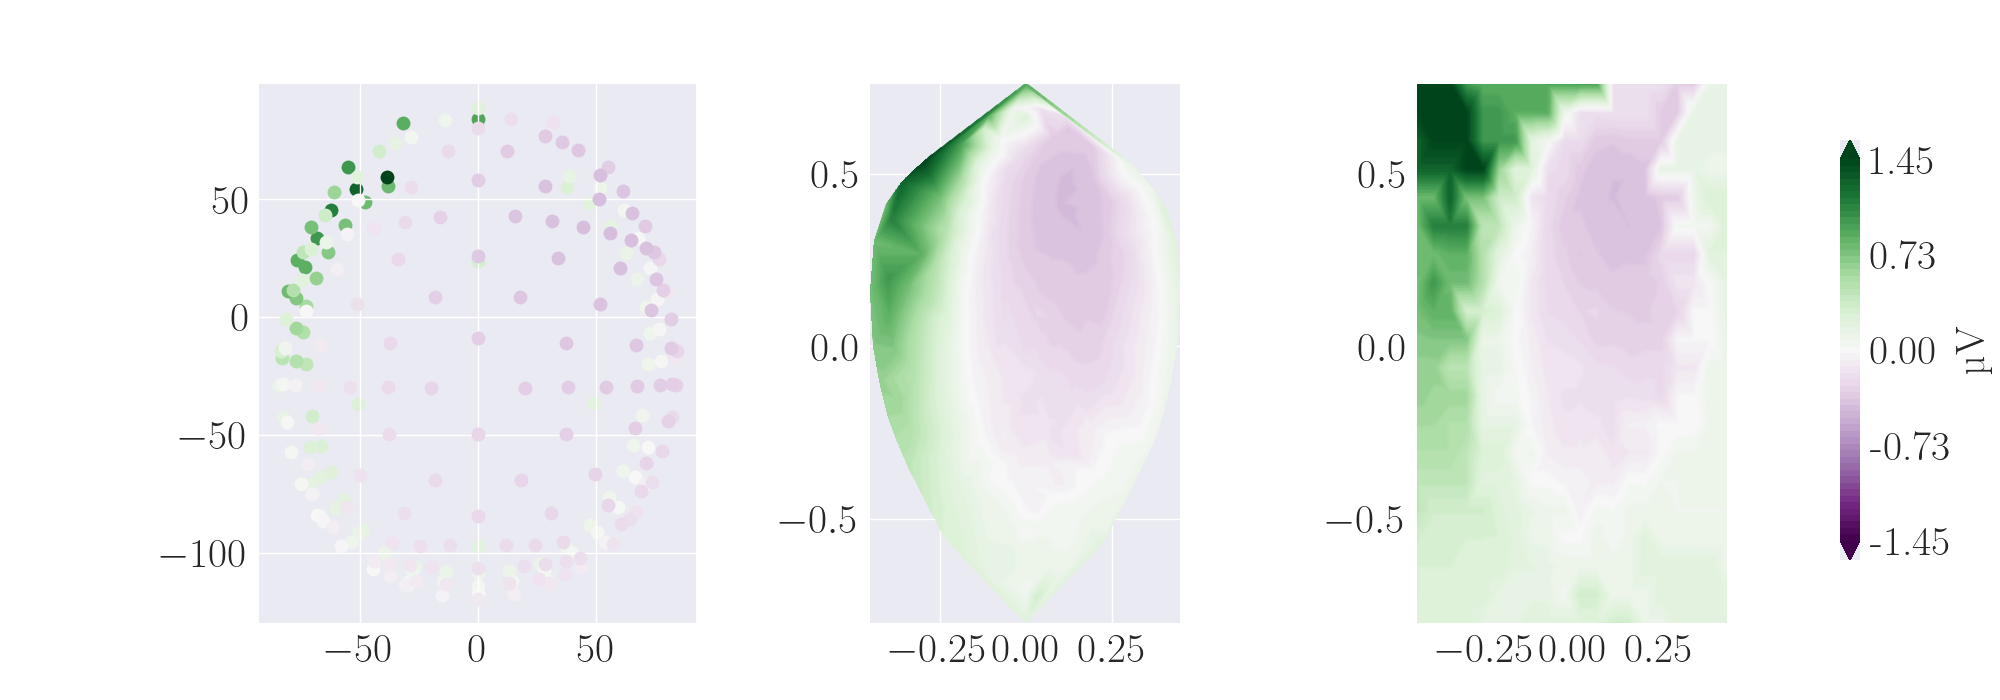
\includegraphics[width=\linewidth]{figures/purple_green/one_dipole_eeg_dipole_pos_1.png}
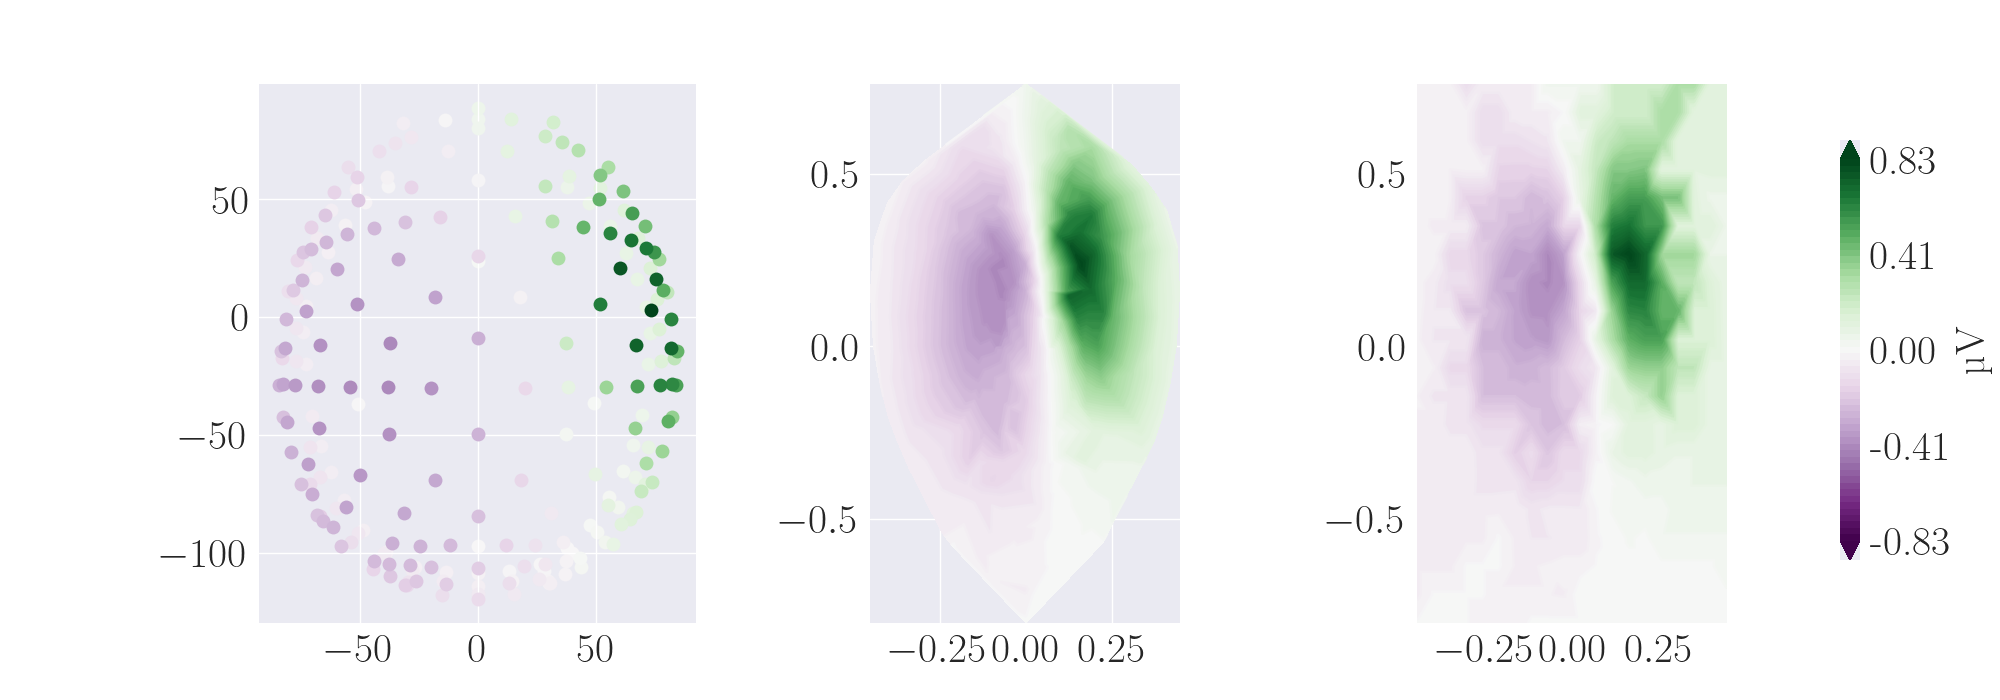
\includegraphics[width=\linewidth]{figures/purple_green/one_dipole_eeg_dipole_pos_3.png}

\caption{\newline
\textbf{Right Panel:} EEG measures for three different samples, expressed in microvolts ($\mu$V). Each sample represents an EEG recording at specific electrode positions. \newline
\textbf{Middle and Left Panels:} Illustration of the interpolation of the EEG data into a two-dimensional matrix. The interpolated data represents the transformation of original electrode recordings into a regular 2D grid, effectively converting the one-dimensional EEG data into an image-like format. The contour plots visualize the spatial distribution of EEG potential intensities, with each point in the matrix corresponding to a specific electrode location.}
\label{fig:eeg_dipole_pos_0}

\end{figure}

\FloatBarrier

\section{Layers in Convolutional Neural Networks}
Convolutional Neural Networks draw inspiration from the information processing mechanisms in the visual cortex of the brain. In the visual cortex, neurons respond selectively to stimuli within specific regions known as receptive fields. This intricate ability allows neurons to effectively capture spatial correlations found in natural images. In the realm of CNNs, this selective response is approximated mathematically using \emph{convolutional operations}, copupled with \emph{pooling layers} and \emph{fully connected layers} \cite{Hjorth-Jensen2022}.

The selective processing observed in the visual cortex is imitated in CNNs by establishing local connections between nodes in a convolutional layer and a subset of nodes from the preceding layer. This stands in contrast to fully connected feed-forward neural networks, where each node connects to every node in the preceding layer. This selective approach enables CNNs to specialize in learning and capturing localized features from input data, such as edges or textures.

A convolution is performed using a \emph{filter}, often described as a small matrix with learnable parameters. Starting from the top-left corner of the input, a filter is systematically positioned over a specific region, depending on its size. At each location, one computes the element-wise product between the filter and the corresponding region of the input data, subsequently summing these products to yield a single value representing the convolution result at that position. After each computation, the filter shifts to the next position. Once the convolution operation is performed at every possible pixel location, the output elements together constitute the \emph{activation map}. The convolutional processes is repeated for an optional number of filters, generating a new activation map for each filter. Given our EEG input data with dimensions of 20x20x1, using six 5x5 convolutional filters yields an output with dimensions of 16x16 and six channels. In essence, this process reduces the spatial dimensions of the image data while increasing its depth. The convolutional process is visually depicted in Figure \ref{fig:conv_operations}.

\begin{figure}[!htb]
  \centering
  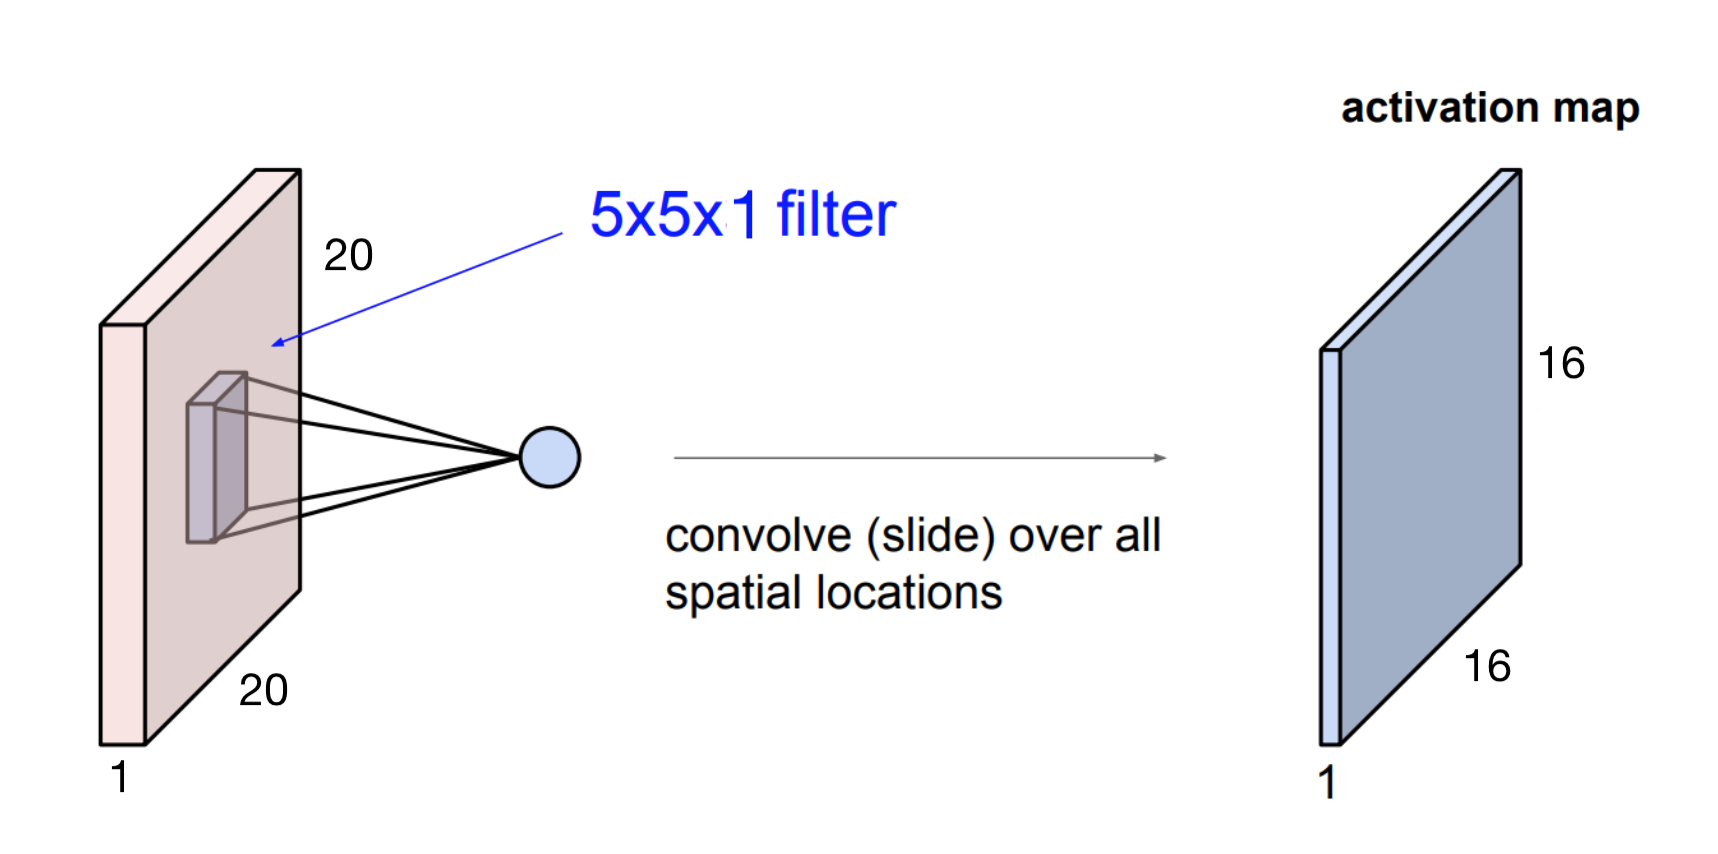
\includegraphics[width=9cm]{figures/Convolutional_operation.png}
  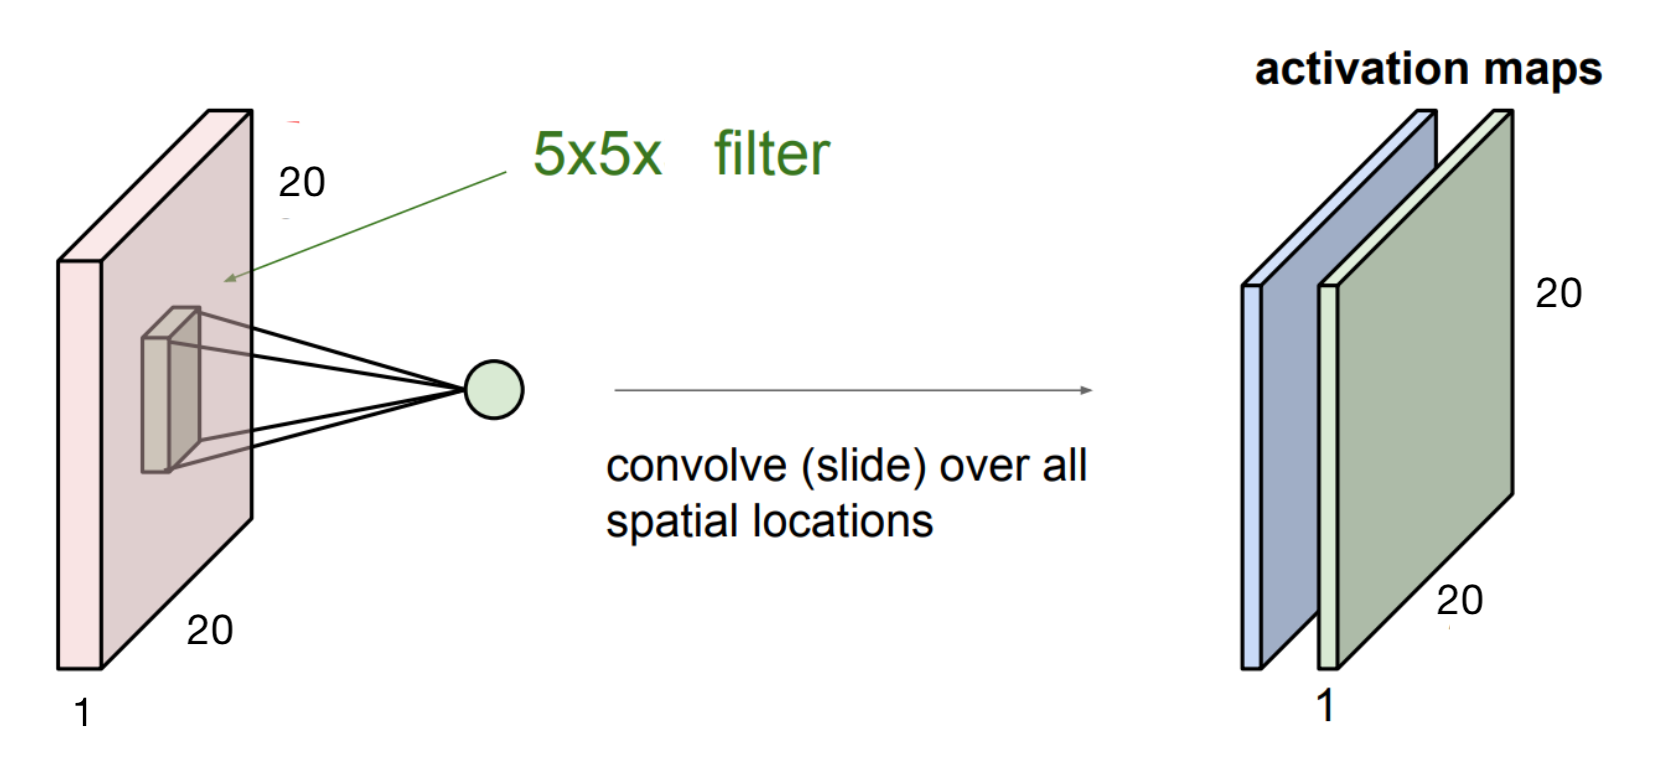
\includegraphics[width=9cm]{figures/conv_operat_2.png}
  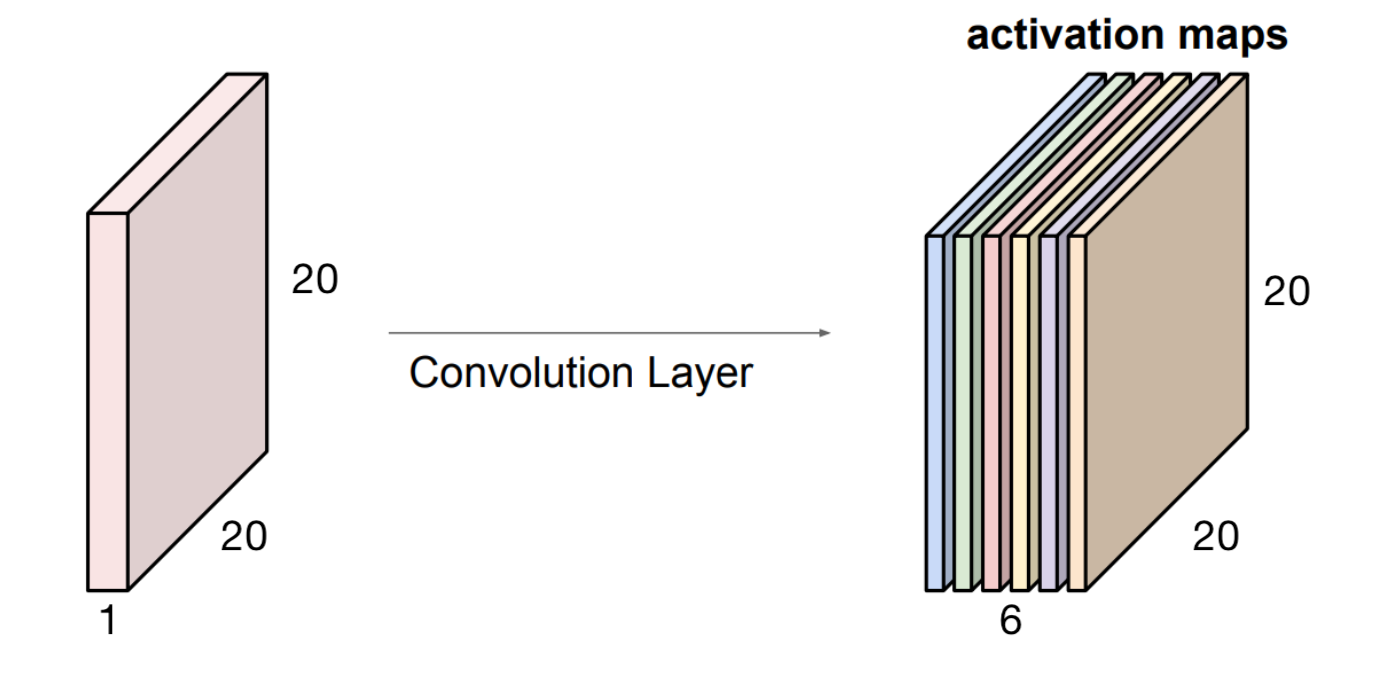
\includegraphics[width=8cm]{figures/conv_operat3.png}
  \caption{Illustration of the convolutional process. The figure has been adapted from Lecture Notes in the course IN5400 from 2021, with attribution to Andreas Kleppe \cite{kleppe-lecture}.}
  \label{fig:conv_operations}
\end{figure}

\FloatBarrier

% \begin{figure}
%   \hspace*{-2cm} % Adjust the value as needed to move the figures left
%   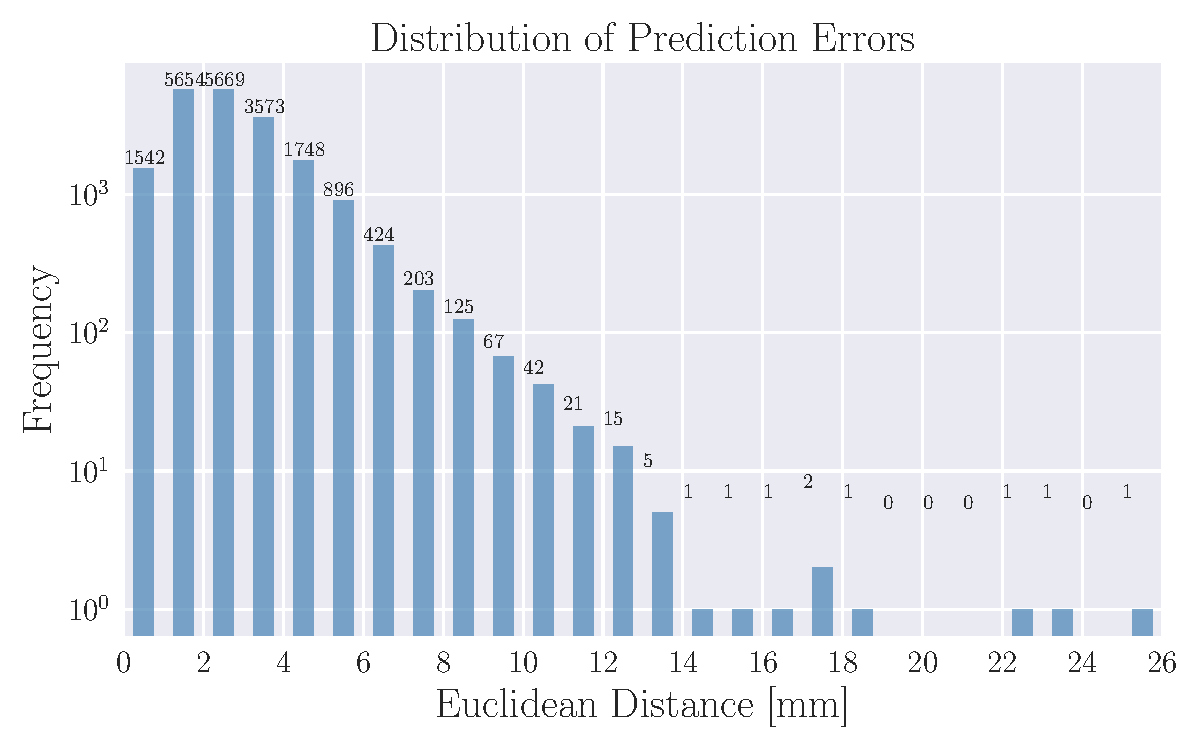
\includegraphics[width=9cm]{figures/new_histogram_position_amplitude.pdf}
%   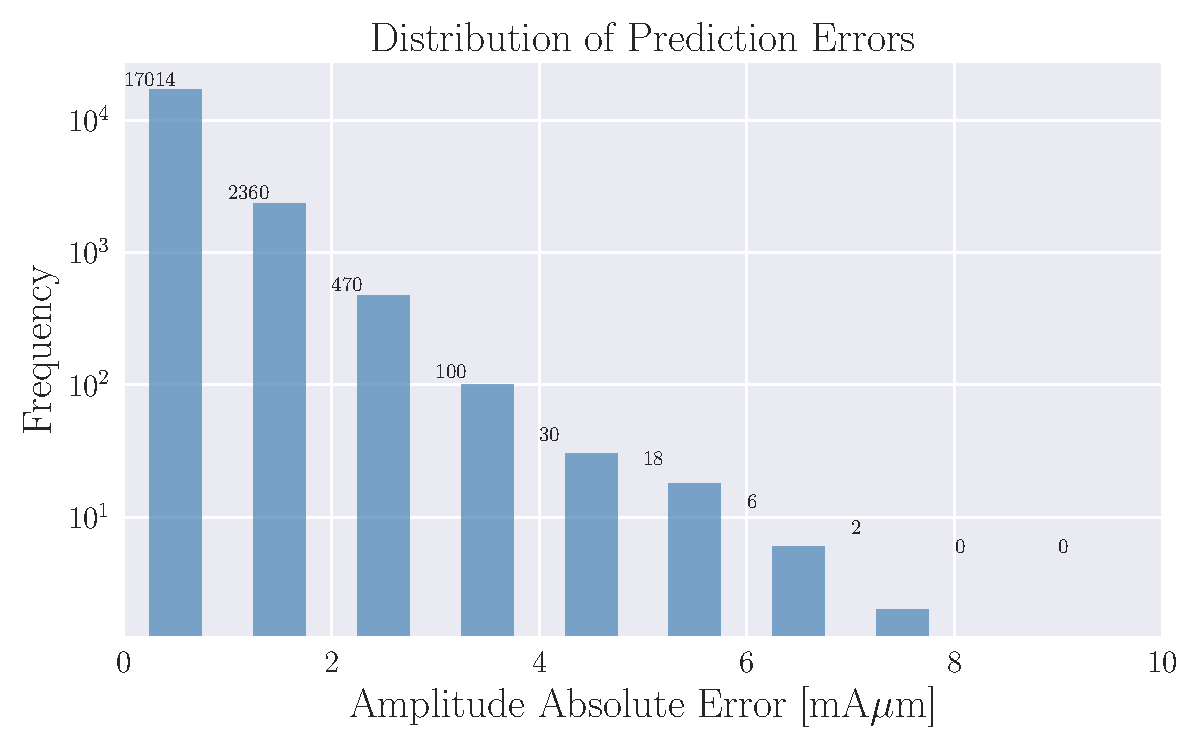
\includegraphics[width=9cm]{figures/new_histogram_amplitude_amplitude.pdf}
%   \caption{Left panel illustrates the distribution of Mean Euclidean Distance for the predicted dipole locations, organized into bins of width 1 mm. Right panel holds the distribution of Mean Absolute Error for the predicted magnitude of dipole electrical signal, presented in a similar format, with bins of width 1 nA$\mu$m.}
%   \label{fig:histogram_magnitude}
% \end{figure}

Following each convolution operation, it is common practice to apply an activation function to each element of the output independently. In our network, we apply the ReLU activation function, as discussed in detail in Chapter 4. The mathematical formulation for each element in the output activation map follows the same structure as in FCNNs:

\begin{equation}
a = f(w^{T}x + b)
\end{equation}

Here, $w$ represents the learnable coefficients within the convolutional filter, $x$ denotes the input, $b$ stands for the bias, $f$ is the activation function, and $a$ symbolizes the output activation map. Importantly, the nature of $w$ differs from the weights in FCNNs; it represents a local spatial region instead of the entire input. Furthermore, $w$ is reused across all spatial regions, functioning as a pattern detector applied in a \emph{position-independent} manner. Consequently, convolutional layers entail considerably fewer trainable parameters compared to their fully connected counterparts, which are prevalent in FCNNs \cite{IN5400-Lecture3}.

\rednote{fix cite}
Following the convolutional layers commonly is the pooling layers. Pooling operations reduce the size of activation maps by the use of a max pooling function that in some sense works very much like a discrete convolution \cite{dumoulin2018}. The max pooling function replaces the linear combination in the convolutional layers with a strided maximum filtering. This method simply chooses the maximum value inside the filter spatial region. By sliding a pooling filter of optional size with a specified \emph{stride}, which determines how much the filter shifts over the input, the highest pattern detector response over the field of view is selected. In this way, spatial information is removed, and the dimension is further decreased.


\section{Architecture, Hyperparameters and Training}

The first layer in our constructed CNN, is a 2D convolutional layer. This layer takes an input image with one channel and applies six distinct filters, each of size 5x5. These filters are responsible for learning specific spatial patterns and detecting relevant features within the input image. As a result of this convolutional operation, the output tensor's spatial dimensions reduce to 16x16, and the depth becomes 6, signifying the extraction of 6 distinct feature maps. Following the convolution layer, a Max Pooling layer, with kernel size 2x2 and stride 1 is employed. This pooling layer aims to downsample the spatial dimensions of the feature maps while preserving the most salient features. The pooling operation reduces the spatial resolution to 15x15, and the depth remains unchanged at six. Next, a second 2D convolutional layer, takes the six-channel output from the previous pooling layer. This layer employs 16 filters of size 5x5, extracting a more complex hierarchy of features from the input data. The output tensor from this layer has spatial dimensions of 11x11 and a depth of 16, signifying the presence of 16 distinct feature maps. Following another Max Pooling layer is employed. Similar to the previous pooling operation, this layer further downsamples the spatial dimensions while preserving the depth, resulting in a feature map size of 10x10 with 16 channels. Further, the output from the last pooling layer is flattened into a one-dimensional vector. This process collapses the spatial dimensions of the feature maps, resulting in a 1D tensor of size 1600 (10x10x16). After flattening, the network proceeds with three fully connected, dense, layers. These layers are responsible for incorporating global context and making high-level abstractions from the learned features. The first fully connected layer, consists of 120 nodes, followed by 64 nodes. Lastly, we have the output layer with three output nodes, corresponding to the three coordinates of the source generating the EEG signal. In Figure \ref{fig:architecture_CNN}, we have provided an illustration of the architecture of the Convolutional neural network.

ReLU activation function is applied after each convolutional and pooling layer, as well as between the fully connected layers. This ReLU activation facilitates the network's ability to capture and propagate complex, nonlinear relationships in the learned features. However, in the output layer, a linear transformation is employed without the use of an activation function in order to enable the neural network to provide direct and unconstrained predictions for the $x$-, $y$-, and $z$-coordinates of the desired dipole source.

Throughout the convolutional network, the weights of the fully connected layers are initialized using the Xavier normal distribution, a method that was also employed in the design of the simple FCNN, as described in Chapter 4. This initialization strategy contributes to the convergence and training stability of the network, ensuring it effectively learns and generalizes from the provided EEG data.

% On later point, discuss how batch size = 64 might have led to less loiser convergence.
The training process for the CNN follows techniques similar to those applied for the simple FCNN, as extensively detailed in Chapter 5. To ensure effective learning and optimal predictions, we employ stochastic gradient descent with momentum as the optimizer, alongside a customized cost function based on the mean Euclidean distance. During training, mini-batches of size 32 are utilized to introduce data variability and prevent the network from converging to local minima. The CNN also maintains a learning rate of 0.001, weight decay of 0.5 and a momentum of 0.35, consistent with the settings used for the FCNN. To facilitate convergence, a learning rate scheduling approach is adopted, gradually reducing the learning rate during training to strike a balance between rapid initial convergence and fine-tuning in later stages. Following the training process, a rigorous evaluation of the CNN's performance is conducted on an independent test data set, providing an unbiased assessment of its predictive accuracy and its ability to generalize to novel data.

\begin{figure}[!htb]
    \hspace*{-3cm} % Adjust the value here to move the figure more to the left
    \centering
    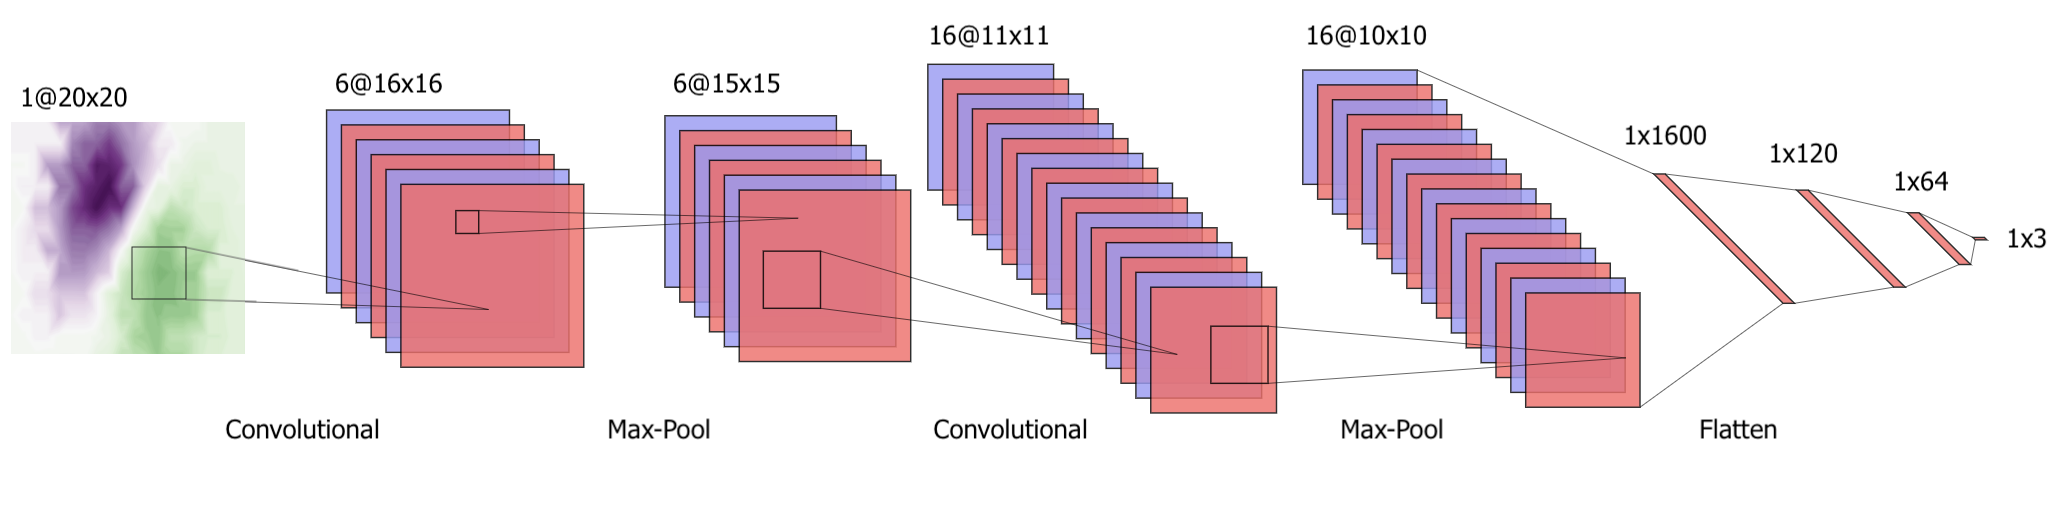
\includegraphics[scale=0.52]{figures/CNN.png}
    \caption{Architecture of the Convolutional Neural Network for localizing single current dipoles. \\
            The visualization has been created using the NN-SVG tool, which was adapted from LeNail (2019) and is licensed under the Creative Commons Attribution 4.0 International License \cite{lenail2019}.}
    \label{fig:architecture_CNN}
\end{figure}

% \FloatBarrier

\rednote{Dele inn i flere subsections slik som i forrige kapittel?}
\section{Performance Evaluation}
Figure \ref{fig:single_dipole_accuracy} illustrates the convergence of the mean Euclidean distance loss. The neural network underwent 600 training epochs, with each training epoch lasting approximately 25 seconds. This resulted in a total training time of approximately 4 hours. It is important to note that this duration encompasses data loading and preprocessing steps. Notably, the CNN required longer epoch times compared to the previously studied FCNN. This difference can be attributed to the additional data preparation and interpolation required to suit the CNN's architecture. In contrast, the simpler FCNN had quicker epochs since its data was already in the desired format, with preprocessing mainly involving data scaling and splitting.

Figure \ref{fig:accuracy_CNN} reveals that both training and validation losses appeared to stabilize between 400 and 600 epochs. Prior to this phase, there were noticeable fluctuations in validation loss, which gradually subsided as the network approached convergence. The figure suggests that the model did not exhibit signs of overfitting, as both training and validation losses consistently decreased. At the final epoch, the training loss measures 1.460 mm, while the validation loss stabilizes at 2.280 mm.

Additionally, Figure \ref{fig:accuracy_CNN_targets} provides insights into the evolution of validation loss concerning individual target coordinates across training epochs. This figure offers information similar to what was observed for the FCNN, indicating that all individual target coordinates carried a roughly similar weight, resulting in comparable loss values for each coordinate. Furthermore, it demonstrates that the fluctuations in loss observed before the 400th epoch disappeared beyond this point, signifying stabilization in loss across all three target coordinates. Notably, the $x$-coordinate exhibited the lowest loss, followed by the $y$-coordinate, while the $z$-coordinate stabilized at the highest loss, consistent with observations from the FCNN. We emphasize, however, that these differences are small and may not be statistically significant in the context of our primary interest.


\begin{figure}[!htb]
    \centering
    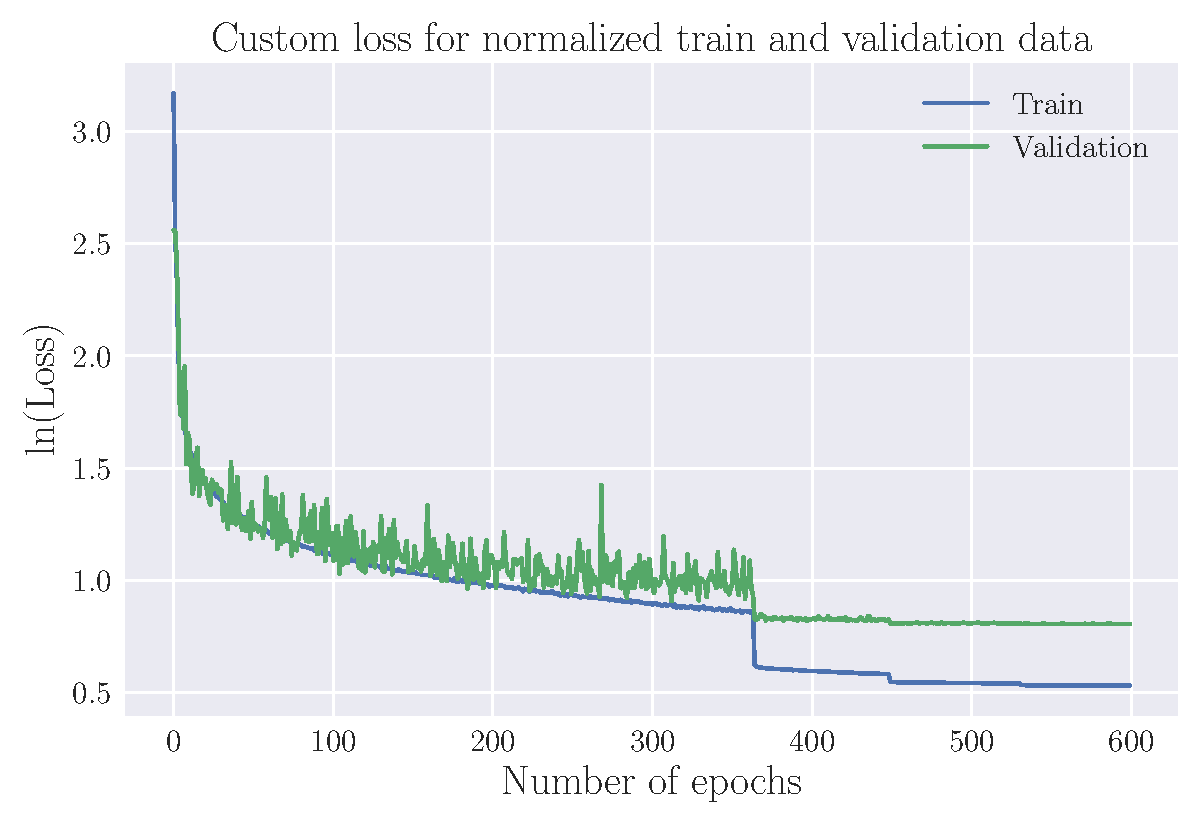
\includegraphics[width=\linewidth]{figures/CNN/Custom_Loss_simple_last_run_old_std_cnn_32_0.001_0.35_0.5_0_600_(0).pdf}
    \caption{Training- and validation MED loss for the convolutional neural network with 50,000 samples and tanh as activation function.}
    \label{fig:accuracy_CNN}
\end{figure}

\begin{figure}[!htb]
    \centering
    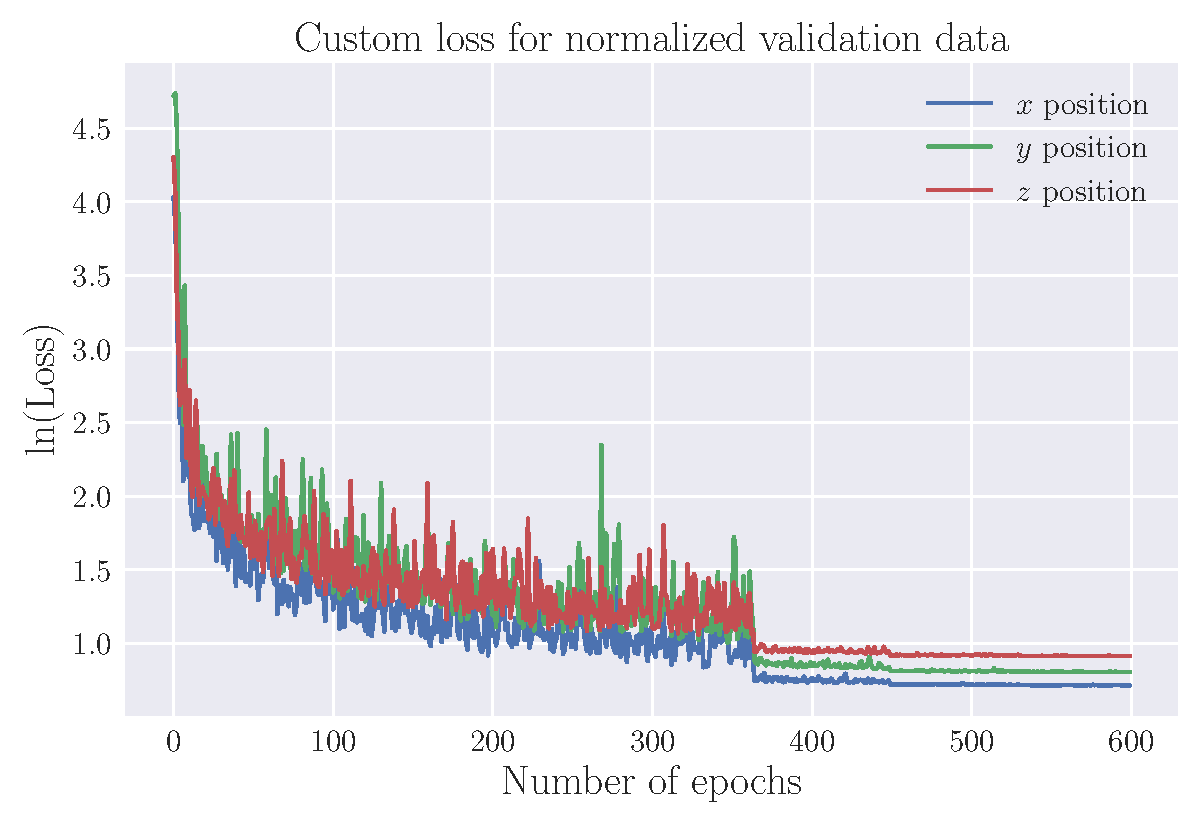
\includegraphics[width=\linewidth]{figures/CNN/Custom_Loss_mse_targets_simple_last_run_old_std_cnn_32_0.001_0.35_0.5_0_600_(0).pdf}
    \caption{Training- and validation MED loss for the convolutional neural network with 50,000 samples and tanh as activation function.}
    \label{fig:accuracy_CNN_targets}
\end{figure}


%\subsection{Position Spesific Performance}
\rednote{Add histogram instead of table?}
The mean Euclidean distance of the CNN's predictions on the unseen test data is measured at 1.80 mm. In Table \ref{ch-conv-table:MED}, we have presented the percentages of samples falling within various Euclidean distance threshold values. Notably, the network exhibits outstanding predictive accuracy, with more than 99.993$\%$ of the samples within the test data set having predictions accurate to within 15 mm. Furthermore, the network achieves a performance exceeding 99.815$\%$ for the 10 mm threshold Euclidean distance values. Approximately 98.030$\%$ of the predictions exhibit an Euclidean distance smaller than 5 mm, a notable achievement that places the CNN's performance just slightly behind the results obtained with the simple FCNN.


\begin{table}[]
  \centering
\begin{tabular}{|ccc|}
\hline
\rowcolor[HTML]{CBCEFB}
\multicolumn{3}{|c|}{\cellcolor[HTML]{CBCEFB}\textbf{Euclidean Distance for Test Samples}}                                                             \\ \hline
\rowcolor[HTML]{EFEFEF}
\multicolumn{1}{|c|}{\cellcolor[HTML]{EFEFEF}ED \textless 5 mm} & \multicolumn{1}{c|}{\cellcolor[HTML]{EFEFEF}ED \textless 10 mm} & ED \textless 15 mm \\ \hline
\rowcolor[HTML]{FFFFFF}
\multicolumn{1}{|c|}{\cellcolor[HTML]{FFFFFF}98.030 $\%$}       & \multicolumn{1}{c|}{\cellcolor[HTML]{FFFFFF}99.815 $\%$}        & 99.993$\%$        \\ \hline
\end{tabular}
\caption{\textbf{ED between targets and predictions of test samples; Predicting Single Dipole Locations with a CNN} \newline
Performance of the network on the test data set comprising 20,000 samples, presented as the percentage of samples falling within ED thresholds of 5 mm, 10 mm and 15 mm respectively.}
\label{ch-conv-table:MED}
\end{table}

\FloatBarrier


Table \ref{ch-conv-table:error_simple_dipole} presents the results for various error metrics associated with the network's predictions. The MAE values for the $x$, $y$, and $z$ coordinates fall within a narrow range, from 0.864 mm to 0.919 mm. These findings indicate that, on average, the network's predictions exhibit an error of less than 1 mm in each coordinate, a level of precision consistent with that achieved by the FCNN.

The MSE values, ranging from 1.579 mm$^2$ to 1.638 mm$^2$, are slightly higher than those observed with the FCNN. However, these values are still relatively small, signifying high performance. The marginally higher MSE values might indicate a slightly broader spread of errors compared to the previous FCNN. To further assess accuracy, we computed the RMSE values, which range from 1.257 mm to 1.280 mm.

Among the three coordinates, the $z$-coordinate exhibits the highest MAE. This observation suggests that the network faces greater challenges in accurately predicting the $z$-coordinate of the dipole source, as indicated earlier in Figure \ref{fig:accuracy_CNN_targets}. However, the $y$ coordinate holds the highest MSE, indicating slightly more significant deviations between predicted and true coordinates compared to the other target coordinates.

For an overall assessment of positional errors, the table provides the average values for MAE, MSE, and RMSE across the three spatial coordinates. These averaged error values remain small, reinforcing also the convolutional neural network's precision in predicting dipole locations for the inverse problem.

\begin{table}[!htb]
\begin{tabular}{l|cccc|}
\cline{2-5}
\rowcolor[HTML]{CBCEFB}
\cellcolor[HTML]{FFFFFF}                           & \multicolumn{4}{c|}{\cellcolor[HTML]{CBCEFB}{\color[HTML]{000000} \textbf{Error Metrics for Target Values}}}                                                                                                                                                                                                                                                                                                                                                     \\ \cline{2-5}
\rowcolor[HTML]{EFEFEF}
\cellcolor[HTML]{FFFFFF}\textbf{}                  & \multicolumn{1}{l|}{\cellcolor[HTML]{EFEFEF}\begin{tabular}[c]{@{}l@{}}$x$-coordinate\\ {[}mm{]}\end{tabular}} & \multicolumn{1}{l|}{\cellcolor[HTML]{EFEFEF}\begin{tabular}[c]{@{}l@{}}$y$-coordinate \\ {[}mm{]}\end{tabular}} & \multicolumn{1}{l|}{\cellcolor[HTML]{EFEFEF}\begin{tabular}[c]{@{}l@{}}$z$-coordinate \\ {[}mm{]}\end{tabular}} & \multicolumn{1}{l|}{\cellcolor[HTML]{EFEFEF}\begin{tabular}[c]{@{}l@{}}Position \\ Error {[}mm{]}\end{tabular}} \\ \hline
\multicolumn{1}{|l|}{\cellcolor[HTML]{EFEFEF}MAE}  & \multicolumn{1}{c|}{0.0.864}                                                                                  & \multicolumn{1}{c|}{0.911}                                                                                   & \multicolumn{1}{c|}{0.919}                                                                                   & 0.898                                                                                                              \\ \hline
\multicolumn{1}{|l|}{\cellcolor[HTML]{EFEFEF}MSE}  & \multicolumn{1}{c|}{1.579}                                                                                  & \multicolumn{1}{c|}{1.710}                                                                                   & \multicolumn{1}{c|}{1.638}                                                                                   & 1.643                                                                                                              \\ \hline
\multicolumn{1}{|l|}{\cellcolor[HTML]{EFEFEF}RMSE} & \multicolumn{1}{c|}{1.257}                                                                                  & \multicolumn{1}{c|}{1.308}                                                                                   & \multicolumn{1}{c|}{1.280}                                                                                   & 1.282                                                                                                              \\ \hline
\end{tabular}
\caption{\textbf{Evaluation of the CNN's performance utilizing different Error Metrics.} \newline
CNN performance on test data set consisting of 20,000 samples. The errors are measured using Mean Squared Error (MSE), Mean Absolute Error (MAE), and Root Mean Squared Error (RMSE).}
\label{ch-conv-table:error_simple_dipole}
\end{table}


To assess the network's performance, we examine a prediction for the same sample within the test set, as we did when evaluating the FCNN. For the dipole located at $\tilde{x} = 66.5$ mm, $\tilde{y} = -26.5$ mm, and $\tilde{z} = 41.9$ mm, the network predicts the coordinates to be $x = 66.4$ mm, $y = -27.3$ mm, and $z = 41.5$ mm. The predicted values closely align with the true values, showing an error of 0.1 mm in the $x$-coordinate, 0.8 mm in the $y$-coordinate, and 0.4 mm in the $z$-coordinate, resulting in a Euclidean distance of 0.99 mm. In Figure \ref{fig:prediction_example}, we have plotted the predicted position $\mathbf{r}$ of the dipole alongside the target position $\mathbf{\tilde{r}}$.

\begin{figure}
  % \hspace*{-2.5cm}
  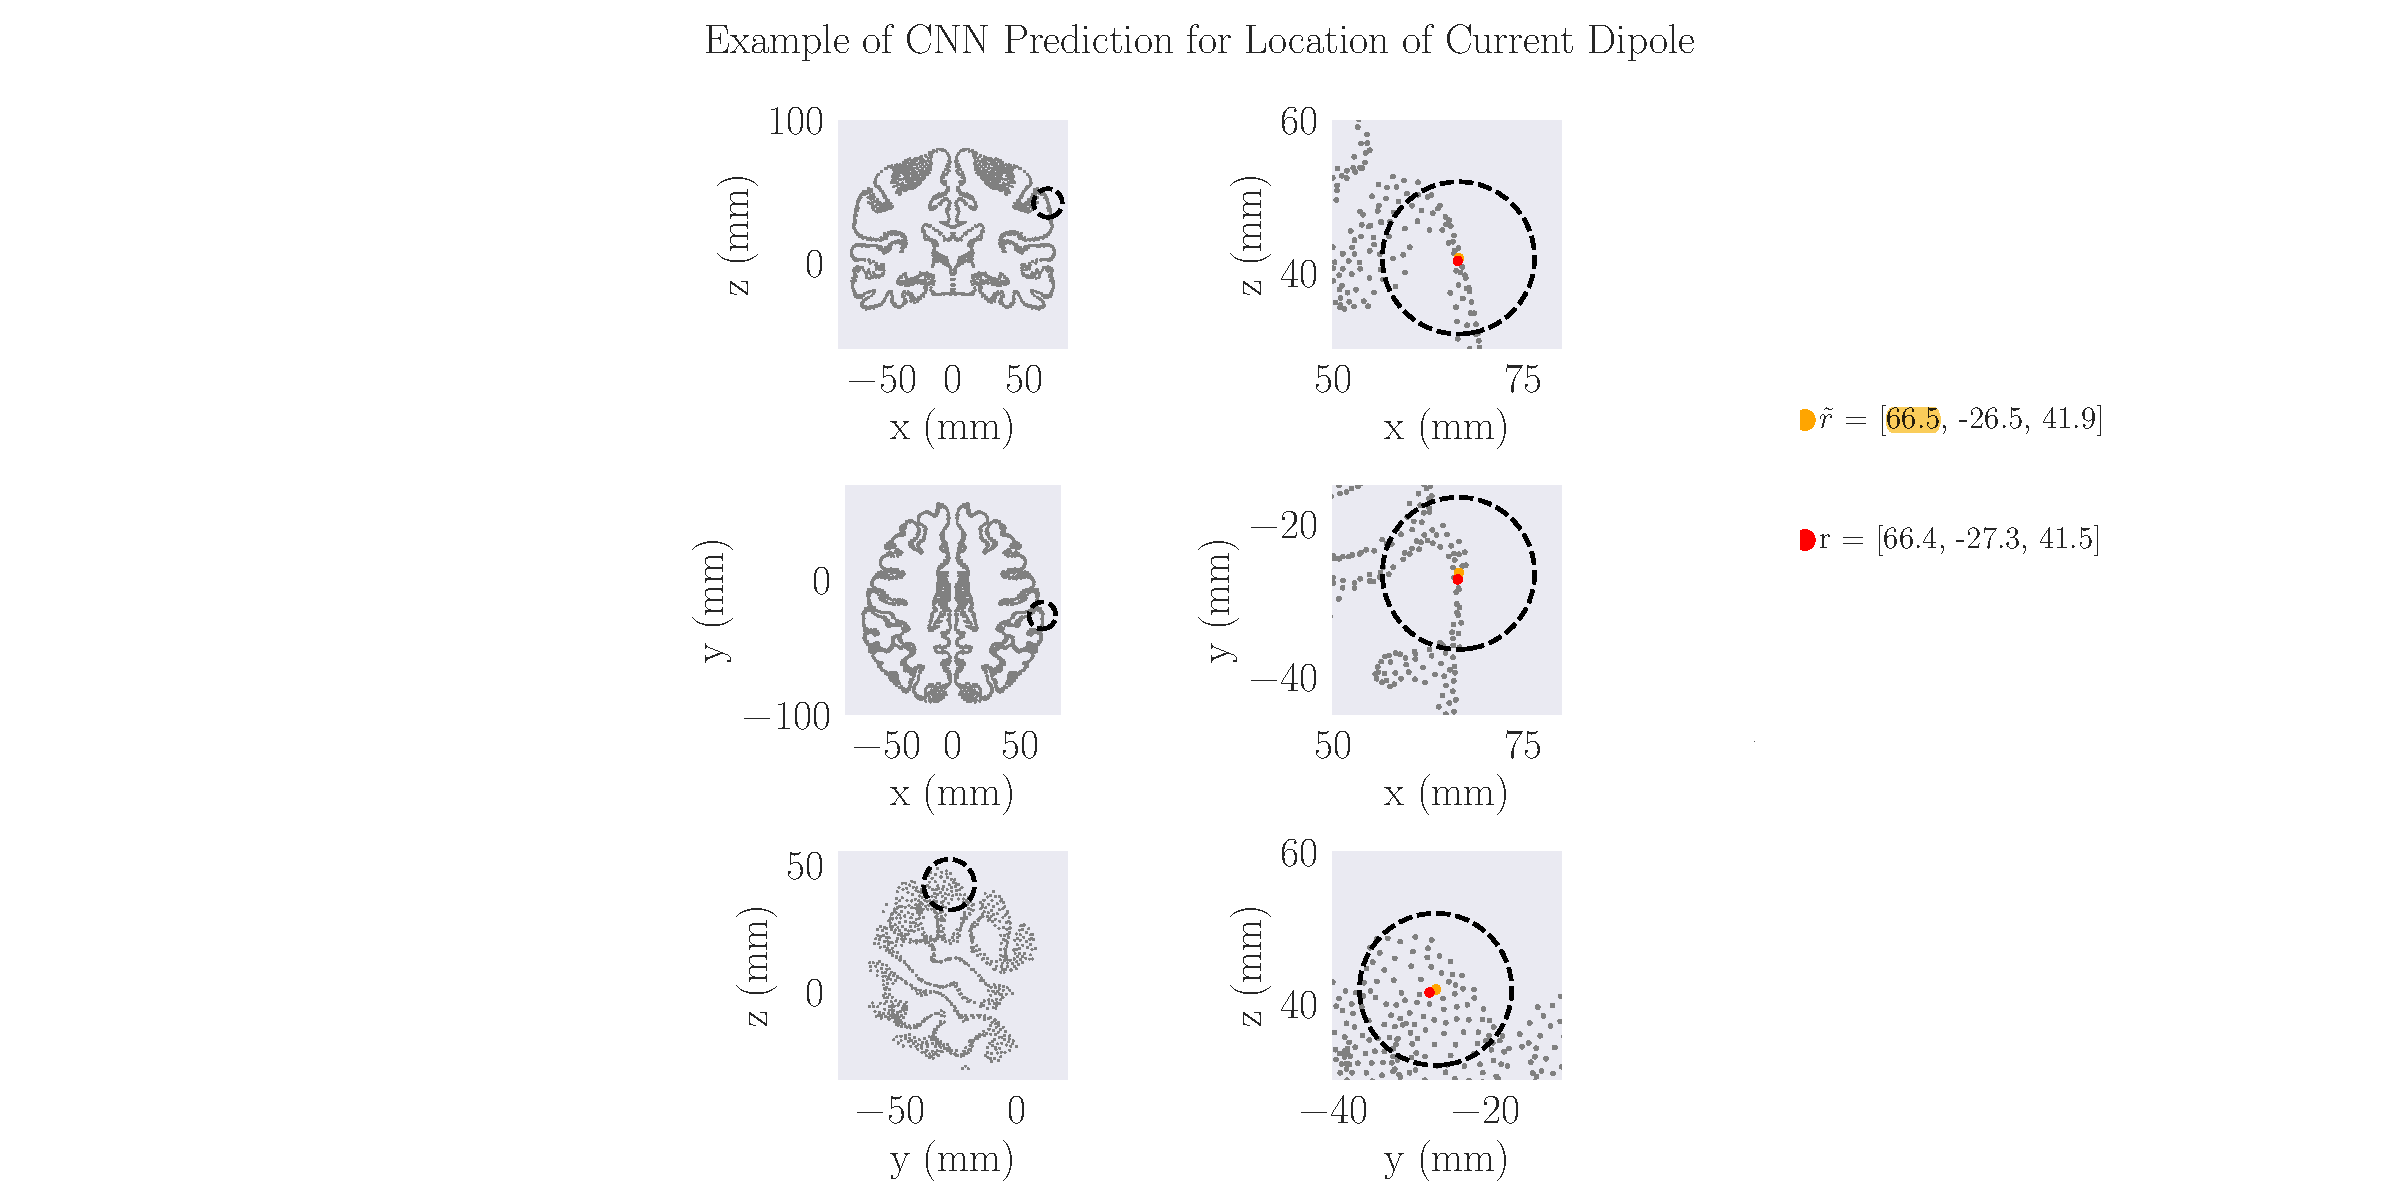
\includegraphics[width=\linewidth]{figures/CNN/single_dipole_prediction.pdf}
  \caption{The CNN's predicted position $r$ of a dipole within the test data set and the target position $\tilde{r}$ The target dipole is marked in orange and the predicted position is marked by a red dot.}
  \label{fig:prediction_example}
\end{figure}




\end{document}
